%% LyX 2.0.3 created this file.  For more info, see http://www.lyx.org/.
%% Do not edit unless you really know what you are doing.
\documentclass[twoside,english]{paper}
\usepackage{lmodern}
\renewcommand{\ttdefault}{lmodern}
\usepackage[T1]{fontenc}
\usepackage[latin9]{inputenc}
\usepackage[a4paper]{geometry}
\geometry{verbose,tmargin=3cm,bmargin=2.5cm,lmargin=2cm,rmargin=2cm}
\usepackage{color}
\usepackage{babel}
\usepackage{float}
\usepackage{bm}
\usepackage{amsthm}
\usepackage{amsmath}
\usepackage{amssymb}
\usepackage{graphicx}
\usepackage{esint}
\usepackage[unicode=true,pdfusetitle,
 bookmarks=true,bookmarksnumbered=false,bookmarksopen=false,
 breaklinks=false,pdfborder={0 0 0},backref=false,colorlinks=false]
 {hyperref}
\usepackage{breakurl}
\usepackage{makeidx}

\makeatletter

%%%%%%%%%%%%%%%%%%%%%%%%%%%%%% LyX specific LaTeX commands.
%% Because html converters don't know tabularnewline
\providecommand{\tabularnewline}{\\}

%%%%%%%%%%%%%%%%%%%%%%%%%%%%%% Textclass specific LaTeX commands.
\numberwithin{equation}{section}
\numberwithin{figure}{section}

%%%%%%%%%%%%%%%%%%%%%%%%%%%%%% User specified LaTeX commands.
\usepackage{babel}

\@ifundefined{showcaptionsetup}{}{%
 \PassOptionsToPackage{caption=false}{subfig}}
\usepackage{subfig}
\makeatother

\usepackage{listings}


\begin{document}

\title{Generalised parton distributions}

\author{Valerio Bertone}

\tableofcontents{}

\section{Introduction}

In this set of notes I collect the technical aspects concerning
generalised parton distributions (GPDs). Since the computation GPDs
introduces new kinds of convolution integrals, a strategy aimed at
optimising the numerics needs to be devised.

\section{Evolution equation}

The evolution equation for GPDs reads:\footnote{It should be noticed
  that the integration bounds of the integration in
  Eq.~(\ref{eq:eveq}) are dictated by the operator defintion of the
  distribution $f$ on the light cone and not by the kernel
  $\mathbb{P}$.}
\begin{equation}\label{eq:eveq}
\mu^2\frac{d}{d\mu^2}f(x,\xi) = \int_{-1}^{1}\frac{dx'}{\left|2\xi\right|}\mathbb{P}\left(\frac{x}{\xi},\frac{x'}{\xi}\right)f(x',\xi)\,.
\end{equation}
In general, the GPD $f$ and the evolution kernel $\mathbb{P}$ should
be respectively interpreted as a vector and a matrix in flavour
space. However, for now, we will just be concerned with the integral
in the r.h.s. of Eq.~(\ref{eq:eveq}) regardless of the flavour
structure.

The support of the evolution kernel
$\mathbb{P}\left(\frac{x}{\xi},\frac{x'}{\xi}\right)$ is shown in
Fig.~\ref{fig:GPDIntDomain}.
\begin{figure}[h]
  \begin{centering}
    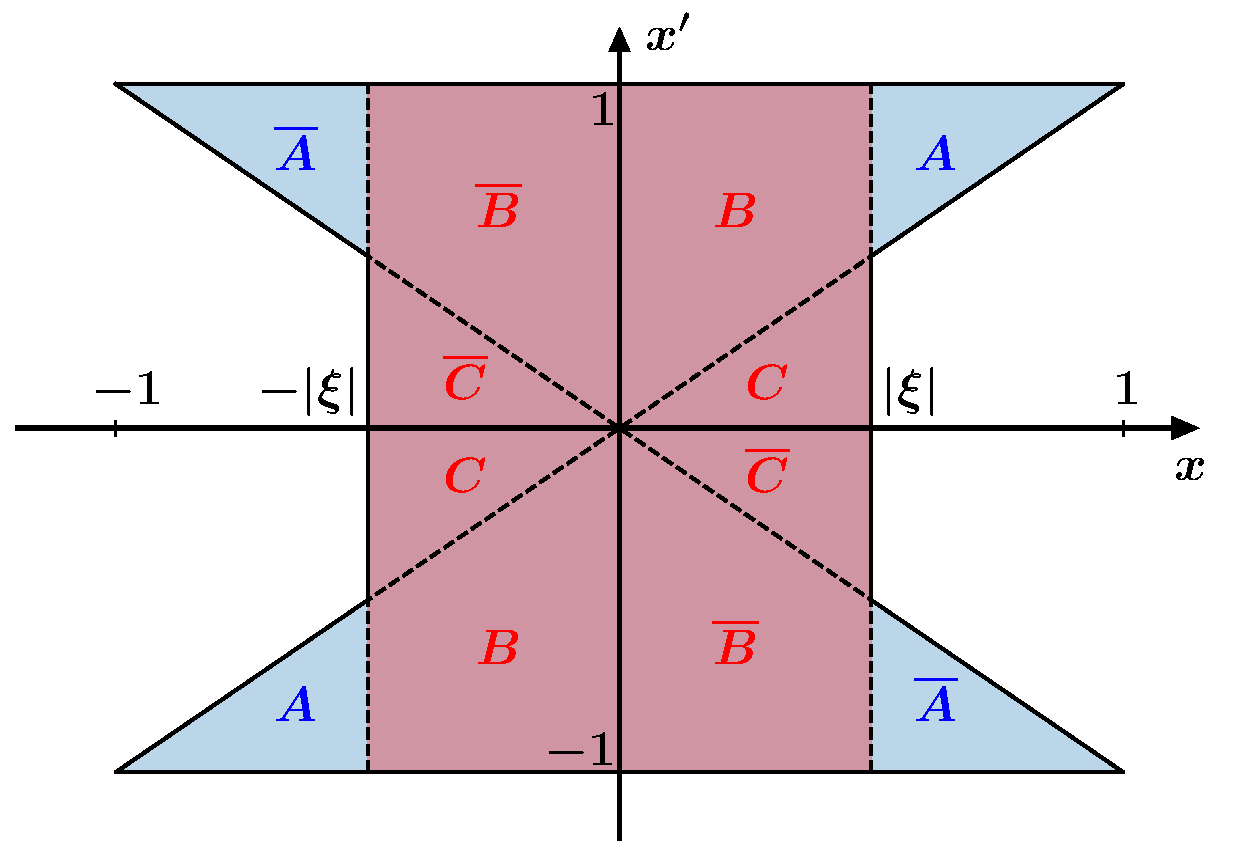
\includegraphics[width=0.7\textwidth]{plots/GPDIntDomain}
    \caption{Support domain of the evolution kernel
      $\mathbb{P}\left(\frac{x}{\xi},\frac{x'}{\xi}\right)$.\label{fig:GPDIntDomain}}
  \end{centering}
\end{figure}
The Knowledge of the support region of the evolution kernel allows us
to rearrange Eq.~(\ref{eq:eveq}) as follows:
\begin{equation}
\displaystyle\mu^2\frac{d}{d\mu^2}f(\pm x,\xi) =\int_{b(x)}^{1}\frac{dx'}{x'}\left[\frac{x'}{\left|2\xi\right|}\mathbb{P}\left(\pm \frac{x}{\xi},\frac{x'}{\xi}\right)f(x',\xi)+\frac{x'}{\left|2\xi\right|}\mathbb{P}\left(\mp \frac{x}{\xi},\frac{x'}{\xi}\right)f(-x',\xi)\right]\,,
\end{equation}
with:
\begin{equation}\label{eq:lowintb}
b(x) = |x|\theta\left(\left|\frac{x}{\xi}\right|-1\right)\,,
\end{equation}
and where we have used the symmetry property of the evolution kernels:
$\mathbb{P}(y,y')=\mathbb{P}(-y,-y')$. In the unpolarised case, it is
useful to define:\footnote{Notice the seemingly unusual fact that
  $f^{+}$ is defined as difference and $f^{-}$ as sum of GPDs computed
  at opposite values of $x$. This can be understood from the fact
  that, in the forward limit, $f(-x)= -\overline{f}(x)$, \textit{i.e.}
  the PDF of a quark computed at $-x$ equals the PDF of the
  corresponding antiquark computed at $x$ with opposite sign. The
  opposite sign is absent in the longitudinally polarised case.}
\begin{equation}\label{eq:pmdef}
\begin{array}{rcl}
\displaystyle f^{\pm}(x,\xi) &=&\displaystyle  f(x,\xi) \mp
                       f(-x,\xi)\,,\\
\\
\displaystyle \mathbb{P}^{\pm}(y,y') &=&\displaystyle  \mathbb{P}(y,y') \mp \mathbb{P}(-y,y')\,,
\end{array}
\end{equation}
so that the evolution equation for $f^{\pm}$ reads:
\begin{equation}\label{eq:eveq2}
\displaystyle\mu^2\frac{d}{d\mu^2}f^{\pm}(x,\xi) = \int_{b(x)}^{1}\frac{dx'}{x'}\frac{x'}{\left|2\xi\right|}
                                                         \mathbb{P}^{\pm}\left(\frac{x}{\xi},\frac{x'}{\xi}\right)f^{\pm}(x',\xi)\,.
\end{equation}
The $f^{\pm}$ distributions can be regarded as the GPD analogous of
the $\pm$ forward distributions that can then be used to construct the
usual singlet and non-singlet distributions in the QCD evolution
basis. This uniquely determines the flavour structure of the evolution
kernels $\mathbb{P}^{\pm}$.

It is relevant to observe that the presence of the $\theta$-function
in the lower integration bound $b$, Eq.~(\ref{eq:lowintb}), is such
that for $|x|>|\xi|$ the evolution equation has the exact form of the
DGLAP evolution equation which corresponds to integrating over the
blue regions in Fig.~\ref{fig:GPDIntDomain} (DGLAP region,
henceforth). Conversely, for $|x|\leq|\xi|$ the lower integration
bound becomes zero and the evolution equation assumes the form of the
so-called ERBL equation that describes the evolution of meson
distribution amplitudes (DAs). This corresponds to integrating over
the red region (ERBL region, henceforth). Crucially, in the limits
$\xi\rightarrow 0$ and $\xi\rightarrow \pm1$ Eq.~(\ref{eq:eveq2})
needs to recover the DGLAP and ERBL equations, respectively.

GPD anomalous dimensions are generally tricky to integrate numerically
because of the intricate support. In order to simplify the integration
procedure, we can decompose the anomalous dimensions using the labels
given in Fig.~\ref{fig:GPDIntDomain} as a guide:
\begin{equation}
\begin{array}{rcl}
\displaystyle\mathbb{P}(y,y')&=&\displaystyle
  \theta(y')\\
\\
&\times&\Big[\theta(y-1)\theta(y'-y)\mathbb{P}_A(y,y')+\theta(1-y)
  \theta(y'-y)\mathbb{P}_B(y,y') +\theta(1-y)
  \theta(y-y')\mathbb{P}_C(y,y')\\
\\
&+&\displaystyle \theta(-y-1)\theta(y+y')\mathbb{P}_{\overline{A}}(y,y')+\theta(1+y)
  \theta(y+y')\mathbb{P}_{\overline{B}} (y,y') +\theta(1+y)
  \theta(-y'-y)\mathbb{P}_{\overline{C}} (y,y')\Big]\\
\\
&+&\displaystyle \theta(-y')\\
\\
&\times&\displaystyle\Big[\theta(y-1)\theta(-y-y')\mathbb{P}_{\overline{A}}(y,y')+\theta(1-y)
  \theta(-y-y')\mathbb{P}_{\overline{B}} (y,y') +\theta(1-y)
  \theta(y'+y)\mathbb{P}_{\overline{C}} (y,y')\\
\\
&+&\displaystyle\theta(-y-1)\theta(-y'+y)\mathbb{P}_A(y,y')+\theta(1+y)
  \theta(-y'+y)\mathbb{P}_B(y,y') +\theta(1+y)
  \theta(-y+y')\mathbb{P}_C(y,y')\Big]\,,
\end{array}
\end{equation}
where the functions $\mathbb{P}_I$ and $\mathbb{P}_{\overline{I}}$,
with $I=A,B,C$, are defined on the respective regions in
Fig.~\ref{fig:GPDIntDomain}.\footnote{Note that $\mathbb{P}_I(y,y')$
  and $\mathbb{P}_{\overline{I}}(y,y')$ are not required to be
  symmetric upon the transformation
  $(y \rightarrow -y, y' \rightarrow -y')$.}  Next, we take the
combinations given in Eq.~(\ref{eq:pmdef}) relevant to implement the
evolution equation in Eq.~(\ref{eq:eveq2}). By doing this, one
obtains:
\begin{equation}\label{eq:DGLAPsuitable}
  \mathbb{P}^\pm(y,y')=\theta(y-1)\mathbb{P}_A^\pm(y,y')+\theta(1-y)
  \left[\theta(y'-y)\mathbb{P}_B^\pm(y,y') +
    \theta(y-y')\mathbb{P}_C^\pm(y,y')\right]\,,
\end{equation}
where we have defined:
\begin{equation}\label{eq:pmdef}
\mathbb{P}_I^{\pm}(y,y') = \mathbb{P}_I(y,y')\mp
\mathbb{P}_{\overline{I}}(-y,y')\,,
\end{equation}
and omitted all the irrelevant/redundant terms and factors for the
computation of the integral in the r.h.s. of
Eq.~(\ref{eq:eveq2}). From Eq.~(\ref{eq:DGLAPsuitable}), it should be
clear that the anomalous dimension $\mathbb{P}_A^\pm$ is responsible
for the evolution in the DGLAP region while $\mathbb{P}_B^\pm$ and
$\mathbb{P}_C^\pm$ are responsible for the evolution in the ERBL
region. The latter observation suggests that $\mathbb{P}_B^\pm$ and
$\mathbb{P}_C^\pm$ are related. The relation can easily be established
by observing that the general structure of the ERBL anomalous
dimensions is:
\begin{equation}
V^{\rm ERBL}(y,y')=\theta(y'-y)F(y,y')+\theta(y-y')F(-y,-y')\,,
\end{equation}
which immediately implies that:
\begin{equation}
\mathbb{P}_C^\pm(y,y')=\mathbb{P}_B^\pm(-y,-y')\,.
\end{equation}
Finally, one finds that a convenient decomposition for the anomalous
dimension in Eq.~(\ref{eq:eveq2}) is:
\begin{equation}
\mathbb{P}^\pm(y,y')=\theta(y-1)\mathbb{P}_A^\pm(y,y')+\theta(1-y)
  \left[\theta(y'-y)\mathbb{P}_B^\pm(y,y') +
  \theta(y-y')\mathbb{P}_B^\pm(-y,-y')\right]\,.
\end{equation}

Eq.~(\ref{eq:eveq2}) can be further manipulated to make it resemble
the structure of the DGLAP equation as much as possible. To this
purpose, we define the parameter:
\begin{equation}
\kappa(x) = \frac{\xi}{x}\,,
\end{equation}
so that:
\begin{equation}\label{eq:manip}
\frac{x'}{\left|2\xi\right|}
\mathbb{P}_I^{\pm}\left(\pm\frac{x}{\xi}, \pm\frac{x'}{\xi}\right)={\rm sign}(\xi)\frac{1}{2\kappa}
\frac{x'}{x} \mathbb{P}_I^{\pm}\left(\pm\frac{1}{\kappa}, \pm\frac{1}{\kappa}
  \frac{x'}{x}\right)\equiv {\rm sign}(\xi)\mathcal{P}_I^{\pm}\left(\pm\kappa,\frac{x}{x'}\right)\,,
\end{equation}
where the last equality effectively defines the \textit{DGLAP-like}
splitting function:
\begin{equation}\label{eq:DGLAPevk}
  \mathcal{P}_I^{\pm}(\pm\kappa,y) = \frac{1}{2\kappa y}
  \mathbb{P}_I^{\pm}\left(\pm\frac{1}{\kappa}, \pm\frac{1}{\kappa y}\right)\,.
\end{equation}
In the following we will assume $\xi>0$ as, so far, this is the only
experimentally accessible region. This allows us to get rid of
${\rm sign}(\xi)$ in Eq.~(\ref{eq:manip}). In addition, without loss
of generality, we can also restrict ourselves to positive values of
$x$ because negative values can be easily accessed by symmetry using
Eq.~(\ref{eq:pmdef}), \textit{i.e.}
$f^{\pm}(-x,\xi)=\mp f^{\pm}(x,\xi)$. Using the definition in
Eq.~(\ref{eq:DGLAPevk}) in the integral in the r.h.s. of
Eq.~(\ref{eq:eveq2}) and finally performing a change of variable
gives:
\begin{equation}\label{eq:DGLAPforGPDs}
\displaystyle\mu^2\frac{d}{d\mu^2}f^{\pm}(x,\xi)= \int_{b(x)}^{1}\frac{dx'}{x'}\mathcal{P}^{\pm}\left(\kappa, \frac{x}{x'}\right)f^{\pm}\left(x',\xi\right)=\int_{x}^{x/b(x)}\frac{dy}{y}\mathcal{P}^{\pm}\left(\kappa,y\right)f^{\pm}\left(\frac{x}{y},\xi\right)\,,
\end{equation}
with:
\begin{equation}
b(x) = x\,\theta(1-\kappa)\,,
\end{equation}
and:
\begin{equation}\label{eq:DGLAPevkdec}
  \mathcal{P}^{\pm}\left(\kappa,y\right)=\theta(1-\kappa)\mathcal{P}_A^\pm(\kappa,y)+\theta(\kappa-1)
  \left[\theta(1-y)\mathcal{P}_B^\pm(\kappa,y) +
    \theta(y-1)\mathcal{P}_B^\pm(-\kappa,y)\right]\,.
\end{equation}
Plugging Eq.~(\ref{eq:DGLAPevkdec}) into Eq.~(\ref{eq:DGLAPforGPDs}),
one obtains:
\begin{equation}\label{eq:DGLAPforGPDs2}
\begin{array}{rcl}
  \displaystyle\mu^2\frac{d}{d\mu^2}f^{\pm}(x,\xi)&=&\displaystyle
                                                      \theta(1-\kappa)\int_{x}^{1}\frac{dy}{y}\mathcal{P}_A^{\pm}\left(\kappa,y\right)f^{\pm}\left(\frac{x}{y},\xi\right)\\
  \\
                                                  &+&\displaystyle\theta(\kappa-1)\int_{x}^{\infty}\frac{dy}{y}\left[\theta(1-y)\mathcal{P}_B^{\pm}\left(\kappa,
                                                      y\right)+\theta(y-1)\mathcal{P}_B^{\pm}\left(-\kappa,y\right)\right]f^{\pm}\left(\frac{x}{y},\xi\right)\,.
\end{array}
\end{equation}
Eq.~(\ref{eq:DGLAPforGPDs2}) has almost the form of a ``standard''
DGLAP equation except for the upper bound of the integral in the
second line that extends up to infinity. However, this kind of
integrals can be handled within APFEL with minor modifications of the
integration strategy and up to a numerical approximation to be
assessed.

\subsection{On continuity of GPDs}

It is well known that GPDs are required to be continuous at $x=\xi$
for factorisation to be valid~\cite{Radyushkin:1997ki}. It is thus
interesting to consider the consequence of this constraint. To this
end, let us consider the limits of Eq.~(\ref{eq:DGLAPforGPDs2}) for
$x\rightarrow \xi^\pm$, which corresponds to
$\kappa\rightarrow 1^{\pm}$:
\begin{equation}\label{eq:limit1}
\lim_{x\rightarrow
  \xi^+}\displaystyle\mu^2\frac{d}{d\mu^2}f^{\pm}(x,\xi) =
\int_{x}^{1}\frac{dy}{y}\mathcal{P}_B^{\pm}\left(1,y\right)f^{\pm}\left(\frac{x}{y},\xi\right)+\int_{1}^{\infty}\frac{dy}{y}\mathcal{P}_B^{\pm}\left(-1,
                                                      y\right)f^{\pm}\left(\frac{x}{y},\xi\right)\,,
\end{equation}
and:
\begin{equation}\label{eq:limit2}
\lim_{x\rightarrow \xi^-}\displaystyle\mu^2\frac{d}{d\mu^2}f^{\pm}(x,\xi) = \mu^2\frac{d}{d\mu^2}f^{\pm}(\xi,\xi)=\int_{x}^{1}\frac{dy}{y}\mathcal{P}_A^{\pm}\left(1,y\right)f^{\pm}\left(\frac{x}{y},\xi\right)\,.
\end{equation}
Taking the difference between Eqs.~(\ref{eq:limit1})
and~(\ref{eq:limit2}), using the continuity of $f^{\rm}$ at $x=\xi$,
and considering that:\footnote{We will prove this equality case by
  case.}
\begin{equation}\label{eq:continuity}
\mathcal{P}_A^{\pm}\left(1,y\right) = \mathcal{P}_B^{\pm}\left(1,y\right)\,,
\end{equation}
one finds:
\begin{equation}
\int_{1}^{\infty}\frac{dy}{y}\mathcal{P}_B^{\pm}\left(-1,
                                                      y\right)f^{\pm}\left(\frac{x}{y},\xi\right)=0\,,
\end{equation}
which has to be valid at any scale and for any $f^{\pm}$. This
immediately implies that:
\begin{equation}\label{eq:contcondition}
\mathcal{P}_B^{\pm}\left(-1, y\right) = 0\,,
\end{equation}
for all values of $y$ and order-by-order in perturbation theory. We
will explicitly verify this constraint when we will discuss the
explicit expressions.

\subsection{End-point contributions}\label{sec:endpoint}

Some of the expressions for the anomalous dimensions discussed below
contain $+$-prescribed terms. It is thus important to treat these
terms properly. We are generally dealing with objects defined as (see
Eq.~(\ref{eq:eveq})):
\begin{equation}
  \frac{1}{|2\xi|}\left[\mathbb{P}\left(\frac{x}{\xi},
      \frac{x'}{\xi}\right)\right]_+=
  \frac{1}{|2\xi|}\mathbb{P}\left(\frac{x}{\xi},
    \frac{x'}{\xi}\right)- \frac{1}{|2\xi|}\delta(x-x')\int_{-\infty}^{\infty}dx'\mathbb{P}\left(\frac{x}{\xi}, \frac{x'}{\xi}\right)\,.
\end{equation}
where the function $\mathbb{P}$ has a pole at $x'=x$. Notice that the
integral in the r.h.s. of the above definition runs over the entire
real axis. It is then the support of the function $\mathbb{P}$ to
possibly redefine the integration bounds. When implementing the
definition in Eq.~(\ref{eq:DGLAPevk}), mostly due to the presence of
the factor $1/y$, one needs to be careful in deriving the appropriate
subtraction term.

Let us take as an example the one-loop non-singlet anomalous
dimension. For definiteness, we will refer for the precise expression
to Eq.~(101) of Ref.~\cite{Diehl:2003ny} and report it here for
convenience (up to a factor $\alpha_s/2\pi$):
\begin{equation}\label{eq:diehlexpr}
V_{\rm NS}^{(0)}(x,x') = 2C_F\left[\rho(x,x')\left\{\frac{1+x}{1+x'}\left(1+\frac{2}{x'-x}\right)\right\}+(x\rightarrow -x, x'\rightarrow -x')\right]_+\,,
\end{equation}
with:\footnote{There is probably a typo in Eq.~(102) of
  Ref.~\cite{Diehl:2003ny} and the second $-1$ should actually be a
  $+1$.}
\begin{equation}\label{eq:supportdiehl}
\rho(x,x')=\theta(-x + x')\theta(1 + x) - \theta(x - x')\theta(1 - x)
\end{equation}
In order for Eq.~(\ref{eq:diehlexpr}) to be consistent with the
forward evolution, one should find:
\begin{equation}\label{eq:forwardlimit}
  \lim_{\xi\rightarrow 0}\frac{1}{|2\xi|} V_{\rm NS}^{(0)}\left(\frac{x}{\xi},\frac{x'}{\xi}\right) \mathop{=}^?
  \frac{1}{x'} P_{\rm NS}\left(\frac{x}{x'}\right) = \frac{1}{x'}2C_F\left[\theta\left(\frac{x}{x'}\right)\theta\left(1-\frac{x}{x'}\right)\frac{1+\left(\frac{x}{x'}\right)^2}{1-\left(\frac{x}{x'}\right)}\right]_+\,,
\end{equation}
such that Eq.~(\ref{eq:eveq}) exactly reduces to the collinear DGLAP
equation. However, if one takes the explicit limit for
$\xi\rightarrow 0$ of Eq.~(\ref{eq:diehlexpr}) one finds:\footnote{The
  factor $\theta\left(\frac{x}{x'}\right)$ comes from the factor
  $\theta(-x+x')$ in Eq.~(\ref{eq:supportdiehl}) that can be rewritten
  as
  $\theta\left(\frac{x}{x'}\right)\theta\left(1-\frac{x}{x'}\right)$.}
\begin{equation}\label{eq:forwardlimit2}
\lim_{\xi\rightarrow 0}\frac{1}{|2\xi|} V_{\rm NS}^{(0)}\left(\frac{x}{\xi},\frac{x'}{\xi}\right) = 2C_F\left[\frac{1}{x'}\theta\left(\frac{x}{x'}\right)\left(1-\frac{x}{x'}\right)\frac{1+\left(\frac{x}{x'}\right)^2}{1-\left(\frac{x}{x'}\right)}\right]_+\,.
\end{equation}
Therefore, as compared to Eq.~(\ref{eq:forwardlimit}), the factor
$1/x'$ in Eq.~(\ref{eq:forwardlimit2}) appears \textit{inside} the
+-prescription sign rather than outside which makes the two
expressions different. The difference amounts to a local term that can
be quantified by knowing that:
\begin{equation}
\left[\theta(y)\theta(1-y)yg(y) \right]_+=y\left[\theta(y)\theta(1-y)g(y)\right]_+ + \delta(1-y)\int_0^1dz\,(1-z)g(z)\,.
\end{equation}
Notice that, thanks to the factor $(1-z)$, the integral in the
r.h.s. of the above equation converges. For example:
\begin{equation}
  \left[y\theta(y)\theta(1-y)\frac{y}{1-y}\right]_+=y\left[\theta(y)\theta(1-y)\frac1{1-y}\right]_+
  + \delta(1-y)\,.
\end{equation}
Finally, one finds that the forward limit of Eq.~(\ref{eq:diehlexpr}) gives:
\begin{equation}\label{eq:forwardlimit}
  \lim_{\xi\rightarrow 0}\frac{1}{|2\xi|} V_{\rm
    NS}^{(0)}\left(\frac{x}{\xi},\frac{x'}{\xi}\right) =
  \frac{1}{x'} \left[P_{\rm NS}\left(\frac{x}{x'}\right)+\frac{4}{3}C_F\delta\left(1-\frac{x}{x'}\right)\right]\,,
\end{equation}
which does \textit{not} reproduce the DGLAP equation due to the
presence of an additional local term. One could reverse the argument
by saying that, in order to reproduce the DGLAP equation, the
well-known expression for the one-loop non-singlet GPD anomalous
dimension misses a local term whose forward limit is $-4C_F/3x$.

\subsection{On Vinnikov's code}

The purpose of this Appendix is to draw the attention on a possible
incongruence of the GPD evolution code developed by Vinnikov and
presented in Ref.~\cite{Vinnikov:2006xw}. For definiteness, we
concentrate on the non-singlet $H_{\rm NS}$ GPD in the DGLAP region
$x>\xi$, whose evolution equation is given in Eq.~(29). For
completeness, I report that equation here:
\begin{equation}\label{eq:Vinnikov}
\begin{array}{rcl}
\displaystyle \frac{d H_{\rm NS}(x,\xi,Q^2)}{d\ln
  Q^2}&=&\displaystyle\frac{2\alpha_s(Q^2)}{3\pi}\Bigg[\int_x^1 dy
          \frac{x^2+y^2-2\xi^2}{(y-x)(y^2-\xi^2)}\left(H_{\rm
          NS}(y,\xi,Q^2)-H_{\rm NS}(x,\xi,Q^2)\right)\\
\\
&+&\displaystyle H_{\rm
    NS}(x,\xi,Q^2)\bigg(\frac32+2\ln(1-x)+\frac{x-\xi}{2\xi}\ln((x-\xi)(1+\xi))\\
\\
&-&\displaystyle \frac{x+\xi}{2\xi}\ln((x+\xi)(1-\xi))\bigg)\Bigg]\,,
\end{array}
\end{equation}
and take the forward limit $\xi\rightarrow 0$:
\begin{equation}\label{eq:Vinnikov}
\begin{array}{rcl}
\displaystyle \frac{d H_{\rm NS}(x,0,Q^2)}{d\ln
  Q^2}&=&\displaystyle\frac{2\alpha_s(Q^2)}{3\pi}\Bigg[\int_x^1 dy
          \frac{x^2+y^2}{y^2 (y-x)}\left(H_{\rm
          NS}(y,0,Q^2)-H_{\rm NS}(x,0,Q^2)\right)\\
\\
&+&\displaystyle H_{\rm  NS}(x,0,Q^2)\left(\frac32+2\ln(1-x)\right)\Bigg]\,,
\end{array}
\end{equation}

The limit for $\xi\rightarrow 0$ of the equation above should
reproduce the usual DGLAP evolution equation:
\begin{equation}
\displaystyle \frac{d H_{\rm 
NS}(x,0,Q^2)}{d\ln
  Q^2}=\frac{\alpha_s(Q^2)}{4\pi}\int_x^1 \frac{dy}{y}\left[\hat{P}_{\rm
  NS}\left(\frac{x}{y}\right)\right]_+H_{\rm NS}\left(y,0,Q^2\right)\,,
\end{equation}
where:
\begin{equation}
\hat{P}_{\rm NS}\left(z\right)=2C_F\frac{1+z^2}{1-z}\,,
\end{equation}
with $C_F=4/3$. Written explicitly and accounting for the additional
local term arising from the incompleteness of the convolution
integral, one finds:
\begin{equation}\label{eq:DGLAPexpl}
\begin{array}{rcl}
  \displaystyle \frac{d H_{\rm NS}(x,0,Q^2)}{d\ln
    Q^2}&=&\displaystyle \frac{2\alpha_s(Q^2)}{3\pi}\Bigg[\int_x^1
            dy\,\frac{x^2+y^2}{y^3(y-x)}\left(y
            H_{\rm NS}\left(y,0,Q^2\right)-xH_{\rm
      NS}(x,0,Q^2)\right)\\
\\
 &+&\displaystyle H_{\rm NS}(x,0,Q^2)\left(\frac{x(x+2)}{2}+2\ln(1-x)\right)\Bigg]\,,
\end{array}
\end{equation}
which evidently differs from Eq.~(\ref{eq:Vinnikov}). By inspection,
one can argue that the difference can be partially traced back to the
issue discussed in Sect.~(\ref{sec:endpoint}). An interesting
observation is that, for $x\rightarrow 1$, the two expressions tend to
coincide. This may have concurred to cause the oversight of this
discrepancy in past numerical comparisons.

\subsection{On Ji's evolution equation}

In this section we discuss the evolution equations derived by Ji in
Ref.~\cite{Ji:1996nm}. This form of the evolution equation is dubbed
``near-forward'' in Ref.~\cite{Blumlein:1999sc} because it closely
resembles the DGLAP equation. However, in Ref.~\cite{Ji:1996nm} two
different equations apply to the regions $x<\xi$ and $x>\xi$. In this
section, we will unify them showing that the resulting one-loop
non-singlet off-forward anomalous dimension cannot be written as a
fully $+$-prescribed distribution.

We start by considering Eqs.~(15)-(17) of Ref.~\cite{Ji:1996nm}. The
first step is to replace $\xi/2$ with $\xi$ to match our
notation. Then we consider the subtraction integrals in Eq.~(16)
keeping in mind that they apply to both regions $x<\xi$ and $x>\xi$,
\textit{i.e.} over the full range in $\kappa$:\footnote{Note that all
  divergent integrals considered here are implicitly assumed to be
  principal-valued integrals such that:
$$
\int_{-1}^{1}\frac{dt}{t}=0\,.
$$
This allows us to omit the $\pm i\epsilon$ terms.}
\begin{equation}
  \int_{\pm \xi}^x\frac{dy}{y-x} = -\int_{\pm \kappa}^1\frac{dz}{1-z}
  = -\int_{0}^1\frac{dz}{1-z}+\int_{1\mp \kappa}^1\frac{dt}{t}=-\int_{0}^1\frac{dz}{1-z}-\ln(|1\mp\kappa|)\,,
\end{equation}
such that the full local term in Eq.~(16) becomes:
\begin{equation}
 \frac{3}{2}+ \int_{\xi}^x\frac{dy}{y-x}+\int_{-\xi}^x\frac{dy}{y-x}
  = \frac{3}{2}-2\int_{0}^1\frac{dz}{1-z}-\ln\left(|1-\kappa^2|\right)\,,
\end{equation}
Considering the symmetry for $\xi\leftrightarrow -\xi$ of the
evolution kernel in Eq.~(17) of Ref.~\cite{Ji:1996nm}, we can write
Eq.~(15) valid for $\kappa<1$ in a more compact way as:
\begin{equation}\label{eq:ji1}
\mu^2\frac{d}{d\mu^2}f^-(x,\xi) = \frac{\alpha_s(\mu)}{4\pi}\int_x^1\frac{dy}{y}\mathcal{P}_1^{-,(0)}(y,\kappa)f^-\left(\frac{x}{y},\xi\right)\,,
\end{equation}
with:
\begin{equation}\label{eq:p1minus0}
\mathcal{P}_1^{-,(0)}(y,\kappa) = 2C_F\left\{\left[\frac{1 +(1-2\kappa^2)y^2}{(1-y)(1-\kappa^2y^2)}\right]_++\delta(1-y)\left[\frac32+\left(\frac{1}{2\kappa^2}-1\right) \ln\left(|1-\kappa^2|\right)+\frac{1}{2\kappa}\ln\left(\left|\frac{1-\kappa}{1+\kappa}\right|\right)\right]\right\}\,.
\end{equation}
The splitting function $\mathcal{P}_1^{-,(0)}$ is such that:
\begin{equation}
\int_0^1dy\,\mathcal{P}_1^{-,(0)}(y,\kappa) =2C_F\left[\frac32+\left(\frac{1}{2k^2}-1\right) \ln\left(|1-\kappa^2|\right)+\frac{1}{2\kappa}\ln\left(\left|\frac{1-\kappa}{1+\kappa}\right|\right)\right]\,,
\end{equation}
which means that it cannot be written as a fully $+$-prescribed
distribution, contradicting, for example, Eq.~(\ref{eq:diehlexpr}).
However, the integral above correctly tends to zero as
$\kappa\rightarrow 0$ allowing one to recover the usual DGLAP
splitting function in the forward limit:
\begin{equation}
  \lim_{\kappa\rightarrow 0}\mathcal{P}_1^{-,(0)}(y,\kappa) = 2C_F\left[\frac{1+y^2}{1-y}\right]_+\,.
\end{equation}

It should also be pointed out that also the limit for
$\kappa\rightarrow 1$ of Eq.~(\ref{eq:p1minus0}) is well-behaved:
\begin{equation}
\lim_{\kappa\rightarrow 1}\mathcal{P}_1^{-,(0)}(y,\kappa) = 2C_F\left\{\left[\frac{1}{1-y}\right]_++\delta(1-y)\left[\frac32-\ln(2)\right]\right\}\,.
\end{equation}
which is required to have a smooth transition from the DGLAP to the
ERBL region.

We now consider Eqs.~(18) and~(19) of
Ref.~\cite{Ji:1996nm} valid for $\kappa>1$. Interestingly, after
some algebra, we find:
\begin{equation}\label{eq:ji2}
\mu^2\frac{d}{d\mu^2}f^-(x,\xi) = \frac{\alpha_s(\mu)}{4\pi}\left[\int_x^1\frac{dy}{y}\mathcal{P}_1^{-,(0)}(y,\kappa)f^-\left(\frac{x}{y},\xi\right)+\int_x^\infty\frac{dy}{y}\mathcal{P}_2^{-,(0)}(y,\kappa)f^-\left(\frac{x}{y},\xi\right)\right]\,,
\end{equation}
with $\mathcal{P}_1^{-,(0)}$ given in Eq.~(\ref{eq:p1minus0}) and:
\begin{equation}\label{eq:p2minus0}
\mathcal{P}_2^{-,(0)}(y,\kappa) = 2C_F(1-\kappa)\frac{y+(1+2\kappa)y^3}{(1-y^2)(1-\kappa^2y^2)}\,.
\end{equation}
It is very interesting to notice that $\mathcal{P}_2^{-,(0)}$ is
proportional to $(1-\kappa)$ that guarantees the continuity of GPDs at
$k=1$.

We observe that, within the integration interval, the splitting
function $\mathcal{P}_2^{-,(0)}$ is singular at $y=1$.\footnote{The
  singularities at $y=-1$ and $y=\pm1/\kappa$ are all placed below
  $y=x$ that is the lower integration bound and thus do not cause any
  problem.} However, as pointed out above, the second integral on the
r.h.s. of Eq.~(\ref{eq:ji2}) has to be regarded as principal-valued
therefore it is well-defined. In order to treat this integral
numerically we consider the specific integral:
\begin{equation}
I=\int_x^\infty dy\,\frac{f(y)}{1-y}\,,
\end{equation}
where $f$ is a test function well-behaved over the full integration
range. If one subtracts and adds back the divergence at $y=1$,
\textit{i.e.}:
\begin{equation}
f(1)\int_0^1dy\,g(y)\,,
\end{equation}
one can rearrange the integral as follows:
\begin{equation}\label{eq:plusplusdist}
I=\int_x^\infty\frac{dy}{1-y}\left[f(y)-f(1)\left(1+\theta(y-1)\frac{1-y}{y}\right)\right]+f(1)\ln(1-x)\equiv
\int_x^\infty dy\left(\frac{1}{1-y}\right)_{++}f(y)\,,
\end{equation}
which effectively defines the $++$-distribution. However, it should be
noticed that this definition is specific to the function $1/(1-y)$. In
case of a different singular function the function that multiplies
$\theta(y-1)$ would be different. The advantage of this rearrangement
is that the integrand is free of the divergence at $y=1$ and is thus
amenable to numerical integration. Also, the $++$-distribution reduces
to the standard $+$-distribution when the upper integration bound is
one rather than infinity. In this sense the $++$-distribution
generalises the $+$-distribution to ERBL-like integrals. However, it
is important to notice that, contrary to the $+$-distribution, the
$++$-distribution does not modify the function it applies to,
specifically:
\begin{equation}
\left(\frac{1}{1-y}\right)_{++} = \frac{1}{1-y}
\end{equation}
for all values of $y$, including $y=1$.

In view of the use of Eq.~(\ref{eq:plusplusdist}), it is convenient to
rewrite Eq.~(\ref{eq:p2minus0}) as follows:
\begin{equation}\label{eq:p2minus01}
  \mathcal{P}_2^{-,(0)}(y,\kappa) =
  2C_F\left[\left(\frac{1}{1-y}\right)_{++}-\frac{1+(1+\kappa)y+(1+\kappa -\kappa^2)y^2}{(1+y)(1-\kappa^2y^2)}\right]\,,
\end{equation}
where the second term in the squared bracket in the r.h.s. is regular
at $y=1$.

Finally, Eqs.~(\ref{eq:ji1}) and Eq.~(\ref{eq:ji2}) can be combined as
follows:
\begin{equation}\label{eq:jitot}
  \mu^2\frac{d}{d\mu^2}f^-(x,\xi) = \frac{\alpha_s(\mu)}{4\pi}\left[\int_x^1\frac{dy}{y}\mathcal{P}_1^{-,(0)}(y,\kappa)f^-\left(\frac{x}{y},\xi\right)+\theta(\kappa-1)\int_x^\infty\frac{dy}{y}\mathcal{P}_2^{-,(0)}(y,\kappa)f^-\left(\frac{x}{y},\xi\right)\right]\,,
\end{equation}
to obtain a singe DGLAP-like evolution equation valid for all values
of $\kappa$.

% \subsection{Valence sum rule}

% The valence sum rule for the GPD $f^-$ reads:
% \begin{equation}\label{eq:sumrule}
% \int_0^1 dx\,f^-(x,\xi) = F\,,
% \end{equation}
% where $F$ is independent of $\mu$ and $\xi$. We now need to check
% whether Eq.~(\ref{eq:jitot}) fullfils these constraints. In doing this
% one need to take into account that the variable $\kappa=\xi/x$ depends
% on $x$.

% \section{Anomalous dimensions}

% A crucial ingredient for an efficient implementation of GPD evolution
% is the availability of the DGLAP-like splitting functions
% $\mathcal{P}_I^{\pm}$, Eq.~(\ref{eq:DGLAPevk}), in a closed form
% amenable to be easily integrated as in Eq.~(\ref{eq:DGLAPforGPDs2}).

% As a first step, we need to make the flavour structure of the
% evolution kernels explicit. Working in the QCD evolution basis, we
% have:
% \begin{equation}
% \mathcal{P}_I^+=\begin{pmatrix}
% P_{I,qq}&P_{I,qg}\\
% P_{I,gq}&P_{I,gg}
% \end{pmatrix}\,,
% \end{equation}
% and:
% \begin{equation}
% \mathcal{P}_I^-=P_I^{\rm NS}\,,
% \end{equation}
% where $P_I^{\rm NS}$ is the appropriate evolution kernel for the
% following particular non-singlet distribution. Each single function
% $P$ admits the perturbative expansion in powers of $\alpha_s$:
% \begin{equation}
%   P(y,\kappa,\mu)=\sum_{n=0}^{\infty}\left(\frac{\alpha_s(\mu)}{4\pi}\right)^{n+1}P^{(n)}(y,\kappa)\,.
% \end{equation}
% At one loop it turns out that all the non-singlet splitting functions
% are equal amongst themselves and to $P_{I,qq}^{(0)}$, \textit{i.e.}
% $P_I^{{\rm NS},(0)}=P_{I,qq}^{(0)}$.\footnote{When going beyond one
%   loop, three different non-singlet structures emerge. In the QCD
%   evolution basis, they are associated to the total-valence and
%   $\pm$-like distributions.}

% Explicit expressions for the one-loop anomalous dimensions can be
% found, for example, in Ref.~\cite{Blumlein:1999sc}. However, these
% expressions require some algebraic manipulation to make them suitable
% for our purpose (se the Mathematica notebook in
% doc/src/codes/GPDKernels.nb). Let us first consider the non-singlet
% unpolarised anomalous dimension at one loop. Using
% Eqs.~(\ref{eq:pmdef}) and~(\ref{eq:DGLAPevk}), one finds:
% \begin{equation}\label{eq:GPDP0}
%   P_I^{{\rm NS},(0)}(\kappa,y) =\left\{
% \begin{array}{ll}
%   I=A: &\displaystyle
%          2C_F\left[\frac{1+(1-2\kappa^2)y^2}{(1-y)(1-\kappa^2 y^2)}\right]_+\,,\\
%   \\
%   I=B: &  \displaystyle
%          2C_F\left[\frac{1}{1-y}+\frac{1-\kappa}{2\kappa}\frac{1}{1+\kappa y}\right]_+\,.
% \end{array}
% \right.
% \end{equation}
% We now verify Eq.~(\ref{eq:continuity}), finding:
% \begin{equation}
% P_A^{{\rm NS},(0)}(1,y) = P_B^{{\rm NS},(0)}(1,y) = 2C_F\left[\frac{1}{1-y}\right]_+\,.
% \end{equation}
% Also Eq.~(\ref{eq:contcondition}) is easily verified:
% \begin{equation}
% P_B^{{\rm NS},(0)}(-1,y) = 0\,.
% \end{equation}
% It is finally interesting to take the DGLAP limit
% $\kappa\rightarrow 0$ of $P_A^{{\rm NS},(0)}$ that gives:
% \begin{equation}
%  P_A^{{\rm NS},(0)}(0,y) = 2C_F\left[\frac{1+y^2}{1-y}\right]_+\,,
% \end{equation}
% that coincides with the usual DGLAP splitting function, as it
% should. Since $P_{I,qq}^{(0)}=P_I^{{\rm NS},(0)}$, the same findings
% apply to $P_{I,qq}^{(0)}$.

% Let us now turn to the remaining splitting functions $P_{I,qg}^{(0)}$,
% $P_{I,gq}^{(0)}$, and $P_{I,gg}^{(0)}$. Their explicit expressions
% read\footnote{The expression for $P_{I,gq}^{(0)}$ derived from
%   Ref.~\cite{Blumlein:1999sc} seems to be wrong because it does not
%   seem to respect the condition in Eq.~(\ref{eq:continuity}). A
%   seemingly correct expression can be found in Ref.~\cite{Ji:1996nm}
%   by performing the replacement $\xi\rightarrow 2\kappa y$ in
%   Eq.~(24).}:
% \begin{equation}\label{eq:GPDP0qg}
%   P_{I,qg}^{(0)}(\kappa,y) =\left\{
% \begin{array}{ll}
%   I=A: & \displaystyle 4 n_f T_R \frac{1 - 2y + (2 - \kappa^2) y^2}{(1 - \kappa^2 y^2)^2}\,,\\
%   \\
% I=B: &  \displaystyle 2n_f T_R \left[\frac{1 + \kappa}{\kappa^2 (1 + \kappa y)}\right] \left[\frac{1 - \kappa}{\kappa y }+\frac{1}{1 + \kappa y}\right]\,,
% \end{array}
% \right.
% \end{equation}
% \begin{equation}\label{eq:GPDP0gq}
%   P_{I,gq}^{(0)}(\kappa,y) =\left\{
% \begin{array}{ll}
% I=A: &  \displaystyle
% 2 C_F \left[\frac{2 - 2y + (1 - \kappa^2) y^2}{y (1 - \kappa^2 y^2)}\right]\,,\\
%   \\
% I=B: &\displaystyle  C_F \left[\frac{2(1+\kappa) - (1 - \kappa^2) y}{\kappa y (1 + \kappa y)}\right]\,,
% \end{array}
% \right.
% \end{equation}
% \begin{equation}\label{eq:GPDP0gg}
%   P_{I,gg}^{(0)}(\kappa,y) =\left\{
% \begin{array}{ll}
% I=A: &  \displaystyle
% 4 C_A\left[ \frac{-2 + y (1 - y + \kappa^2 (1 + y))}{(1 - \kappa^2 y^2)^2}+\frac{1}{y}+\frac1{\left(1-y\right)_+}\right]+\delta(1-x)\frac{11C_A-4n_fT_R}{3}\,,
%   \\
% I=B: &\displaystyle  C_A\left[\frac{-1 + 3 \kappa^2 - 
%    \kappa (2 + (1 - \kappa)^2 \kappa) y}{\kappa^3 y (1 + \kappa y)^2}+\frac{2}{y}+\frac{2}{\left(1-y\right)_+}\right]+\delta(1-x)\frac{11C_A-4n_fT_R}{3}
% \,.
% \end{array}
% \right.
% \end{equation}
% The continuity condition at $\kappa=1$ is obeyed, producing:
% \begin{equation}
%   P_{A,qg}^{(0)}(1,y) = P_{B,qg}^{(0)}(1,y)= \frac{4 n_f T_R}{(1 + y)^2}\,,
% \end{equation}
% \begin{equation}
%   P_{A,gq}^{(0)}(1,y) =P_{B,gq}^{(0)}(1,y)=\frac{4 C_F}{y (1 + y)}\,,
% \end{equation}
% \begin{equation}
%   P_{A,gg}^{(0)}(1,y) =P_{B,gg}^{(0)}(1,y) =4 C_A\left[\frac{1+y^2}{y(1 + y)^2 \left(1-y\right)_+}\right]+\delta(1-y)\frac{11C_A-4n_fT_R}{3}\,,
% \end{equation}
% as well as the condition in Eq.~(\ref{eq:contcondition}) (NOT TRUE FOR
% $P_{gg}$. TO BE CHECKED!). Finally, their forward limit
% ($\kappa\rightarrow 0$) is:
% \begin{equation}
% \begin{array}{l}
%   \displaystyle P_{A,qg}^{(0)}(0,y) = 4 n_f T_R \left[y^2+(1 - y)^2\right] \\
% \\
%   \displaystyle
% P_{A,gq}^{(0)}(0,y) =2 C_F \left[\frac{1+(1 - y)^2}{y}\right]\,,\\
% \\
%   \displaystyle
%   P_{A,gg}^{(0)}(0,y) =4 C_A\left[ -2 + y (1 - y)+\frac{1}{y}+\frac1{\left(1-y\right)_+}\right]+\delta(1-x)\frac{11C_A-4n_fT_R}{3}\,,
% \end{array}
% \end{equation}
% which correctly reproduces the one-loop DGLAP splitting functions.







\newpage

\begin{thebibliography}{alp}

%\cite{Diehl:2003ny}
\bibitem{Diehl:2003ny}
  M.~Diehl,
  %``Generalized parton distributions,''
  Phys.\ Rept.\  {\bf 388} (2003) 41
  doi:10.1016/j.physrep.2003.08.002, 10.3204/DESY-THESIS-2003-018
  [hep-ph/0307382].
  %%CITATION = doi:10.1016/j.physrep.2003.08.002, 10.3204/DESY-THESIS-2003-018;%%
  %1016 citations counted in INSPIRE as of 30 Oct 2019

%\cite{Blumlein:1999sc}
\bibitem{Blumlein:1999sc}
  J.~Blumlein, B.~Geyer and D.~Robaschik,
  %``The Virtual Compton amplitude in the generalized Bjorken region: twist-2 contributions,''
  Nucl.\ Phys.\ B {\bf 560} (1999) 283
  doi:10.1016/S0550-3213(99)00418-6
  [hep-ph/9903520].
  %%CITATION = doi:10.1016/S0550-3213(99)00418-6;%%
  %86 citations counted in INSPIRE as of 13 Feb 2020

%\cite{Radyushkin:1997ki}
\bibitem{Radyushkin:1997ki}
A.~V.~Radyushkin,
%``Nonforward parton distributions,''
Phys. Rev. D \textbf{56} (1997), 5524-5557
doi:10.1103/PhysRevD.56.5524
[arXiv:hep-ph/9704207 [hep-ph]].
%1104 citations counted in INSPIRE as of 02 Jul 2020

%\cite{Ji:1996nm}
\bibitem{Ji:1996nm}
X.~D.~Ji,
%``Deeply virtual Compton scattering,''
Phys. Rev. D \textbf{55} (1997), 7114-7125
doi:10.1103/PhysRevD.55.7114
[arXiv:hep-ph/9609381 [hep-ph]].
%1183 citations counted in INSPIRE as of 08 Jul 2020

%\cite{Vinnikov:2006xw}
\bibitem{Vinnikov:2006xw}
A.~V.~Vinnikov,
%``Code for prompt numerical computation of the leading order GPD evolution,''
[arXiv:hep-ph/0604248 [hep-ph]].
%21 citations counted in INSPIRE as of 20 Jul 2020

\end{thebibliography}

\end{document}
